%%%%%%%%%%%%%%%%%%%%%%%%%%%%%%%% 
\section{The CERN Single-Phase Prototype} 
\label{sec:proto-cern-single}


The CERN single-phase prototype detector is a crucial milestone
towards construction and operation of the first 10~kt DUNE far
detector module. The prototype detector and beam test serves two
principal functions.  The first is to serve as an engineering
prototype to validate the performance of all detector components,
establish and commission production sites and to test the installation
procedure.  The second is to collect and study physics data in
response to charged particles of different type and energy.  Results
from these measurements serve to validate MC simulations, serve as
data input to sensitivity studies of the DUNE experiment and allow to
validate and tune event reconstruction and particle identification
tools.

To mitigate the risks associated with extrapolating small scale
versions of the single-phase LAr TPC technology to a full-scale
detector element, it is essential to benchmark the operation of
full-scale detector elements and perform measurements in a well
characterized charged particle beam.


Many basic detector performance parameters can be established with
cosmic ray muons and the results are critical to inform the production
of the first 10~kt DUNE far detector components. This allows to
identify potentially problematic components and lead to future
improvements and optimizations of the detector design. However, a
well defined charged particle test beam will significantly enhance the
detector performance measurements.  In particular, the following
checks are anticipated:
\begin{enumerate}
 \item characterize performance of full scale TPC module
 \item study performance of the photon detection system
 \item test and evaluate performance of detector calibration tools (e.g. laser system)
  \item verify functionality of cold TPC electronics under LAr cryogenic conditions
  \item perform full-scale structural tests under LAr cryogenic conditions
  \item verify argon contamination levels and associated mitigation procedures
  \item develop and test installation procedures for full-scale detector components
  \item identify flaws and inefficiencies in the manufacturing process
\end{enumerate}

The physics sensitivity of the DUNE experiment has been estimated
based on measured detector performance characteristics published in
the literature, simulation based estimates as well as a variety of
assumptions about the anticipated performance of the future detector
and event reconstruction and particle identification algorithms.  The
proposed single-phase LAr prototype detector and CERN beam test aim to
replace these assumptions with measurements for the full scale DUNE
detector components and the presently available algorithms. Thereby
the measurements will allow enhanced accuracy and reliability of DUNE
physics sensitivity projections.  The beam measurements will serve as
a calibration data set to tune the Monte Carlo simulations and serve
as a reference data set for measurements of the future DUNE detector.
In order to make precise measurements, the detector will need to
accurately identify and measure the energy of the particles produced
in the neutrino interaction with Argon which will range from hundreds
of MeV to several GeV.

More specifically, the goals of the prototype detector beam test measurements include
the use of a charged particle beam to:
\begin{enumerate}
\item measure the detector calorimetric response for
\begin{enumerate}
	\item hadronic showers
	\item electromagnetic showers
\end{enumerate}
\item study e/$\gamma$-separation capabilities
\item measure event reconstruction efficiencies as function of energy and particle type 
\item measure performance of particle identification algorithms as function of energy 
\item assess single particle track calibration and reconstruction
%		-- characterize performance of algorithms
\item validate the accuracy of Monte Carlo simulations in the relevant energy range

%  \item secondary hadron interactions in detector
\item study other topics with the collected data sets
 \begin{enumerate}
    \item pion interaction kinematics and cross sections
    \item kaon interaction cross section to characterize proton decay backgrounds 
    \item muon capture for charge identification
 \end{enumerate}
\end{enumerate}

A detailed estimate enumerating the desired minimum integrated
particle counts as a function of charged particle species and momentum
is nearing completion. This estimate is also converted into a run plan
based on realistic beam composition, particle energies and efficiency
information.

The CERN single-phase detector and beam test program is in preparation
and an invited technical proposal\cite{CERN_single-phase_proposal} to
the CERN SPSC will be submitted in June 2015. The planing foresees to
take a first beam data run in 2018 before the long shutdown of the
LHC. Experiences gained from construction, installation and
commissioning of the CERN single-phase prototype detector as well as
performance tests with cosmic ray data are expected to lead to an
optimization of equivalent phases of the DUNE far detector.

\subsection{Detector Configuration and Components}

Since the CERN single-phase prototype detector serves as an
engineering prototype detector for the first 10~kt module of the
DUNE far detector all components have exactly the same dimensions and
features as those described in section \ref{ch:detectors-fd-ref}. That
is all TPC and photon detector components, as well as their
positioning and spacing within their cryostat are exactly as planned
for the DUNE far detector modules.

\subsubsection{TPC configuration}

The size of the CERN single-phase prototype detector is determined by
the requirement to fully contain hadronic showers of up to several GeV
in energy.  The particle containment of hadronic showers initiated by
charged pions or protons is a critical feature for calorimetric
measurements. Simulation studies indicate that showers initiated by 10
GeV primary pions and protons are contained within a volume measuring
6~m in the longitudinal and 5$\times$5~m$^2$ in the transverse
directions. With the basic APA unit measuring 6$\times$2.3~m$^2$ an
arrangement of two times 3 APAs side-by-side, a central cathode and
two drift volumes with 3.6~drift length each was identified as the
arrangement which satisfies the
requirements. Figure~\ref{fig:CERN_single_TPC} shows a view of the
CERN single phase TPC along with the field cage and also a view of the
TPC within the cryostat.
%
\begin{cdrfigure}[Cutaway view]{CERN_single_TPC}{View of the CERN 
single-phase detector TPC (left) and inserted in the cryostat (right). }
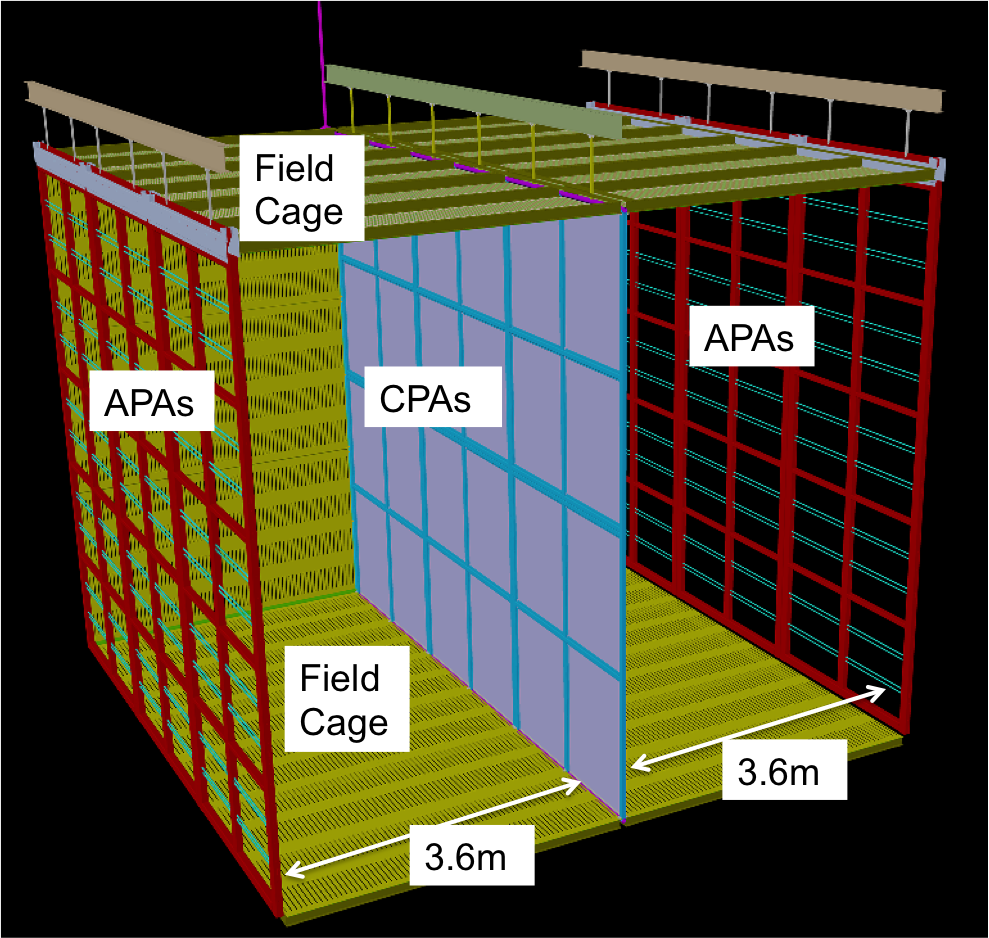
\includegraphics[width=0.40\textwidth]{CERN_single_TPC}
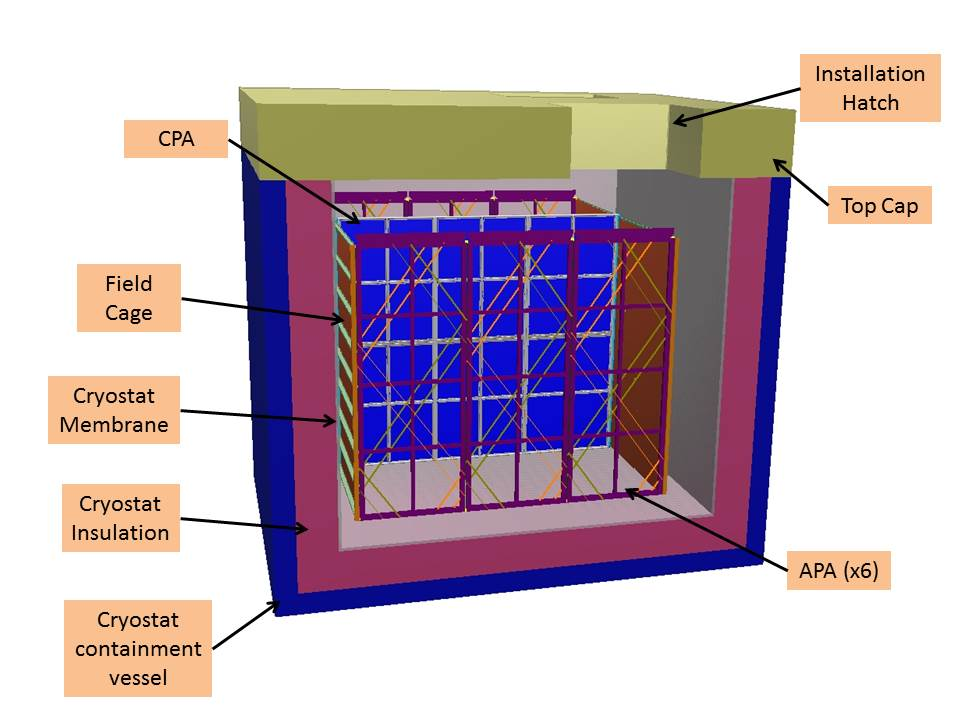
\includegraphics[width=0.59\textwidth]{TPC-3D-section}
\end{cdrfigure}
%
For descriptions of the TPC readout, photon-detection system, DAQ,
slow control and monitoring as well as the key issues of the
installation procedure we refer to the corresponding sections of the
DUNE far detector~\ref{ch:detectors-fd-ref}.

\subsubsection{Cryostat}

The Single-phase TPC test at CERN will use a membrane tank technology
with internal dimensions of 7.8~m (tranverse)$\times$ 8.9~m
(parallel)$\times$8.1~m (height).  It can contain 725~t of LAr,
equivalent to about 520~m$^3$. The active (fiducial) detector mass of
liquid argon amounts to 400~t (300~t).\\ The cryostat design is
based on a scaled up version of the LBNE 35-t
Prototype\cite{montanari_35ton}.  Unlike the 35t cryostat it will use
a steel outer supporting structure with an inside metal liner to
separate the insulation volume. It is similar to the cryostat of the
dual phase prototype detector WA105 and to the Fermilab Short-Baseline
Near Detector. The support structure will rest on I-beams to allow for
air circulation underneath the cryostat in order to maintain the
temperature within the allowable limits.  In this vessel a stainless
steel membrane contains the liquid cryogen. The pressure loading of
the cryogenic liquid is transmitted through rigid foam insulation to
the surrounding outer support structure. The membrane is corrugated to
provide strain relief resulting from temperature related expansion and
contraction. The vessel is completed with a top cap that uses the same
technology.  The external cryostat dimensions are 10.6~m
(tranverse)$\times$ 11.7~m (parallel)$\times$10.9~m (height).


The cryostat top cap consists of the same layers as the cryostat
walls. From the inside out the stainless steel primary membrane,
intermediate insulation layers and vapor barrier all continue across
the top of the detector, and thereby provide a leak tight seal.  The
cryostat roof is a removable steel truss structure to which stiffened
steel plates are welded from the underside. They form a flat vapor
barrier surface onto which the roof insulation attaches directly.

The truss structure rests on the top of the supporting structure where
a positive structural connection between the two is made to resist the
upward force caused by the slightly pressurized argon in the ullage
space. The hydrostatic load of the LAr in the cryostat is carried by
the floor and the sidewalls. In order to meet the maximum deflection
of 3~mm between APA and CPA and to decouple the detector form possible
sources of vibrations, the TPCs will be connected to an external
bridge over the top of the plate supported on the floor of the
building. Everything else within the cryostat (electronics, sensors,
cryogenic and gas plumbing connections) is supported by the steel
plates under the truss structure.

All piping and electrical penetration into the interior of the
cryostat are made through the top plate.  Penetrations are clustered
in one region.  The top cap will have two large openings for TPC
installation, and a manhole to enter the tank after the hatches have
been closed.

\subsubsection{Cryogenic System}

The main goal of the LAr system is to purge the cryostat prior to the
start of the operations (with GAr in an open and a closed loop), cool
down the cryostat and fill it with LAr. Successively the LAr is
continuously purified and the boil off GAr is captured to maintain the
required purity. The design requirement calls for a 10~ms electron
lifetime (30 ppt O$_2$ equivalent), a quantity which is measured by
the detector.

The LAr receiving facility includes a storage dewar and an ambient
vaporizer to deliver LAr and GAr to the cryostat. The LAr goes through
the liquid argon handling and purification system, whereas the Gar
through the gaseous argon purification before entering the vessel.
Studies are ongoing to standardize the filtration scheme and select
the optimal filter medium for all future generation detectors,
including this test prototype.

During operation, an external LAr pump circulates the bulk of the
cryogen through the LAr purification system. The nominal LAr
purification flow rate allows for 5.5 days for a full volume exchange.
The boil off gas is first recondensed and then is sent to the LAr
purification system before re-entering the vessel.

The proposed liquid argon system is based on the design of the LBNE
35-t prototype, the MicroBooNE detector systems and the current plans
for the DUNE single phase far detector.








    
    
